\documentclass[a4paper,12pt]{article}
%\documentclass{Configuration_Files/Template}

%------------------------------------------------------------------------------
%	REQUIRED PACKAGES AND  CONFIGURATIONS
%------------------------------------------------------------------------------

% CONFIGURATIONS
\usepackage{parskip} % For paragraph layout
\usepackage{setspace} % For using single or double spacing
\usepackage{emptypage} % To insert empty pages
\usepackage{multicol} % To write in multiple columns (executive summary)
\setlength\columnsep{15pt} % Column separation in executive summary
\setlength\parindent{0pt} % Indentation
\raggedbottom  

% PACKAGES FOR TITLES
\usepackage{titlesec}
% \titlespacing{\section}{left spacing}{before spacing}{after spacing}
\titlespacing{\section}{0pt}{3.3ex}{2ex}
\titlespacing{\subsection}{0pt}{3.3ex}{1.65ex}
\titlespacing{\subsubsection}{0pt}{3.3ex}{1ex}
\usepackage{color}

% PACKAGES FOR LANGUAGE AND FONT
\usepackage[english]{babel} % The document is in English  
\usepackage[utf8]{inputenc} % UTF8 encoding
\usepackage[T1]{fontenc} % Font encoding
\usepackage[11pt]{moresize} % Big fonts

% PACKAGES FOR IMAGES
\usepackage{graphicx}
\usepackage{transparent} % Enables transparent images
\usepackage{eso-pic} % For the background picture on the title page
\usepackage{subfig} % Numbered and caption subfigures using \subfloat.
\usepackage{tikz} % A package for high-quality hand-made figures.
\usetikzlibrary{}
\graphicspath{{./Images/}} % Directory of the images
\usepackage{caption} % Coloured captions
\usepackage{amsthm,thmtools,xcolor} % Coloured "Theorem"
\usepackage{float}

% STANDARD MATH PACKAGES
\usepackage{amsmath}
\usepackage{amsthm}
\usepackage{amssymb}
\usepackage{amsfonts}
\usepackage{bm}
\usepackage[overload]{empheq} % For braced-style systems of equations.
\usepackage{fix-cm} % To override original LaTeX restrictions on sizes

% PACKAGES FOR TABLES
\usepackage{tabularx}
\usepackage{longtable} % Tables that can span several pages
\usepackage{colortbl}

% PACKAGES FOR ALGORITHMS (PSEUDO-CODE)
\usepackage{algorithm}
\usepackage{algorithmic}

% PACKAGES FOR REFERENCES & BIBLIOGRAPHY
\usepackage[colorlinks=true,linkcolor=black,anchorcolor=black,citecolor=black,filecolor=black,menucolor=black,runcolor=black,urlcolor=black]{hyperref} % Adds clickable links at references
\usepackage{cleveref}
\usepackage[square, numbers, sort&compress]{natbib} % Square brackets, citing references with numbers, citations sorted by appearance in the text and compressed
\bibliographystyle{abbrvnat} % You may use a different style adapted to your field

% OTHER PACKAGES
\usepackage{pdfpages} % To include a pdf file
\usepackage{afterpage}
\usepackage{lipsum} % DUMMY PACKAGE
\usepackage{fancyhdr} % For the headers
\fancyhf{}

%----------------------------------------------------------------------------
%	NEW COMMANDS DEFINED
%----------------------------------------------------------------------------

% EXAMPLES OF NEW COMMANDS
\newcommand{\bea}{\begin{eqnarray}} % Shortcut for equation arrays
\newcommand{\eea}{\end{eqnarray}}
\newcommand{\e}[1]{\times 10^{#1}}  % Powers of 10 notation

%----------------------------------------------------------------------------
%	ADD YOUR PACKAGES (be careful of package interaction)
%----------------------------------------------------------------------------

\usepackage{geometry}
\usepackage{tabularx}
\usepackage{booktabs,xltabular}

%----------------------------------------------------------------------------
%	ADD YOUR DEFINITIONS AND COMMANDS (be careful of existing commands)
%----------------------------------------------------------------------------

% Set uniform margins
\geometry{
  left=0.8in,
  right=0.8in,
  top=1in,
  bottom=1in,
  includehead,
  includefoot
}

\begin{document}
\title{Students\&Company Design Document} % Title Page
\author{Alessandro Salvatore, Erdal Yalçın, Leonardo Ratti}
\date{Academic Year: 2024-25}
\maketitle

\tableofcontents
\newpage

\section{Introduction}
\subsection{Purpose}
This document contains the design description of the Students\&Company system. It includes
the architectural design, the user interface design and the descrpition of the operations
that the system will perform. It also show how the requirements and use cases detailed
in the RASD document are satisfied by the design of the system. \\ \newline 
This document is intended to be read by the developers of the system, the testers and the
project managers. It is also intended to be used as a reference for the future maintenance
of the system.
\subsection{Scope}
The Students\&Company system is a web application that allows companies to advertise internship opportunities
for university students. A recommendation system is used for enhancing the matching possibilities between the two parties.
The system provides also suggestions for students and companies to increase their chances to get matched by the recommendation system. \\ \newline
A more detailed description of the system can be found in the RASD document, whilist in
this document is provided a detailed description of the design of the system to implement
the requirements and use cases described in the RASD document.
\subsubsection{Definitions}
\subsubsection{Acronyms}
\subsubsection{Abbreviations}
\subsection{Revision History}
\subsection{Reference Documents}
\subsection{Document Structure}

\section{Overall Description}
\subsection{Overview: High-level Components and Interaction}
\subsection{Component View}
\subsubsection{Entity Manager}
\subsubsection{ckbSP}
\subsubsection{Logical Description of Data}
\subsection{Deployment View}
We adopted a 3-tier architecture hosted on cloud infrastructure, designed to optimize performance and scalability while reducing costs.

Let's explore more in detail:

\begin{enumerate}
    \item \textbf{Scalability and Flexibility} - the ability to add or remove resources such as virtual machines, performance cores, or memory as needed, in conjunction with the use of load balancing services, allows the servers to adapt to changes in traffic or workload.
    \item \textbf{Security} - Firewalls help to protect the application server against data breaches and other security threats.
    \item \textbf{Cost-efficiency} - the choice of using a cloud provider allows us to only pay for the resources that we are actually using, which can help to lower the overall costs, and in general reduces the waste of resources.
\end{enumerate}

The cloud provider is an ideal choice for hosting large, high-traffic applications. The chosen cloud provider will need to offer all of these features in order to meet our needs.

The web server resides in the De Militarized Zone and is the primary interface for user interaction. The application server executes the core application logic, processing user requests and handling all the operations. Load balancers are implemented to evenly distribute incoming traffic across multiple instances of Web and Application Servers.
\begin{figure}[H]
    \centering
    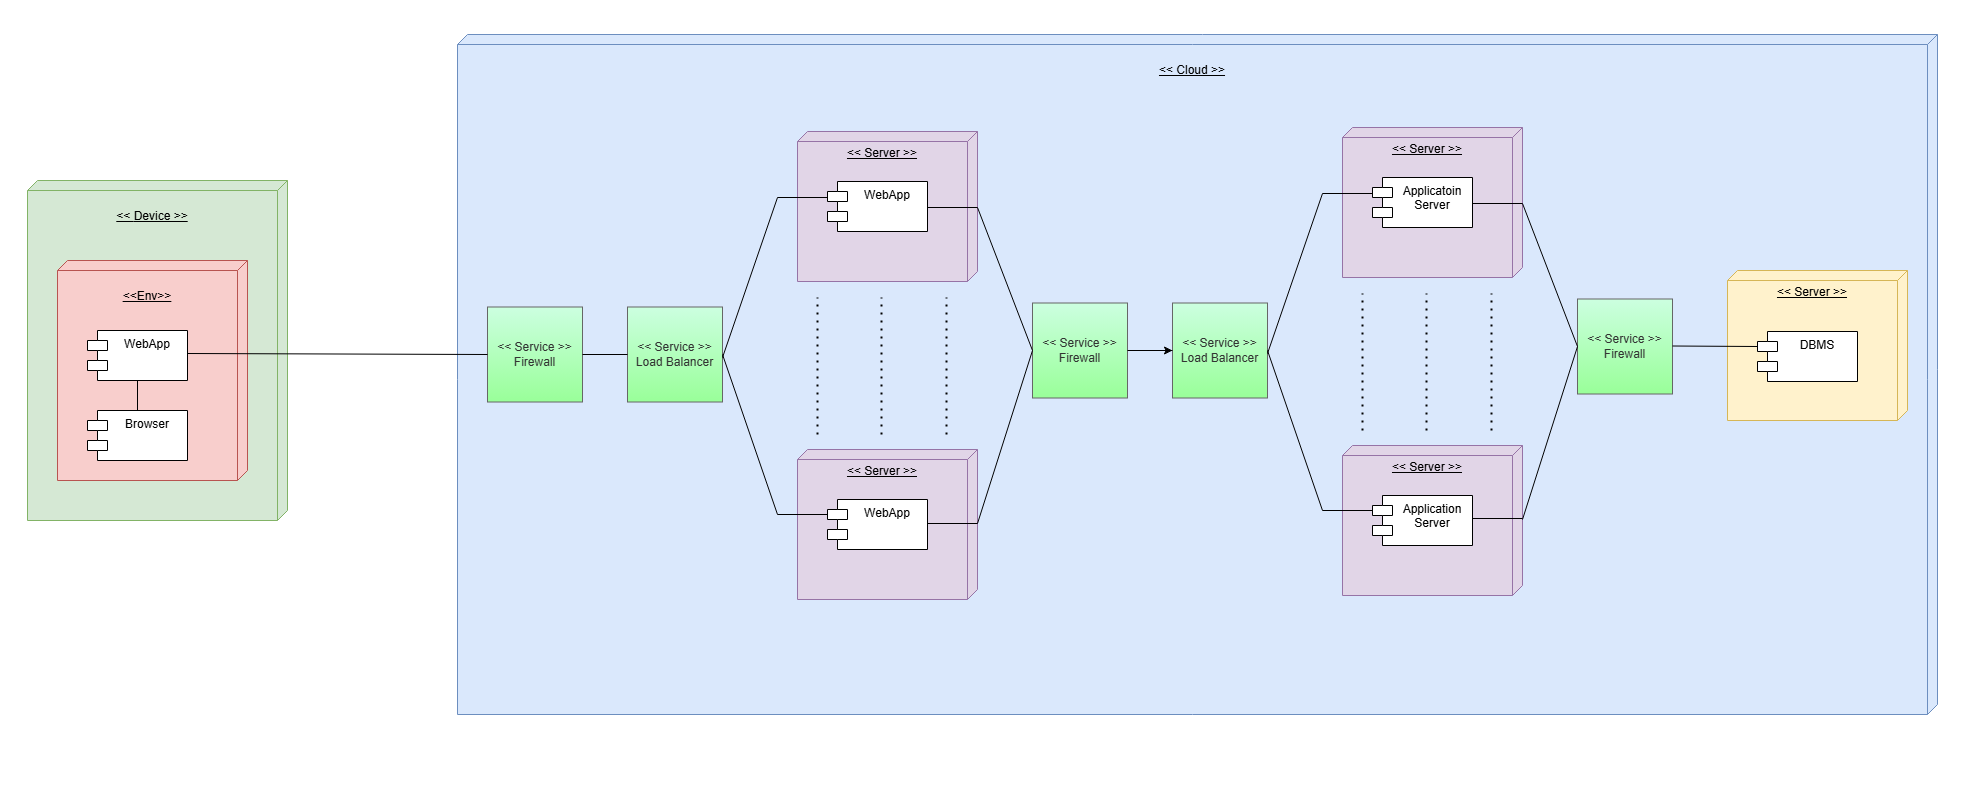
\includegraphics[scale = 0.33]{figures/DD/SingleDiagrams/DeploymentView.png}
    \caption{University Sign Up Page}
    \centering
\end{figure}
\subsection{Runtime View}
\subsection{Component Interfaces}
\subsubsection{API Endpoints}
\subsection{Selected Architectural Styles and Patterns}
\subsection{Other Design Decisions}
\subsubsection{Scale-out}
\subsubsection{Relational Database}
\subsubsection{Token-Based Authentication and Authorization}
\subsubsection{Distributed MVC Pattern}

\section{User Interface Design}

\section{Requirements Traceability}

\section{Implementation, Integration and Testing Plan}
\subsection{Development Process and Approach}
\subsection{Implementation \& Integration Plan}
\subsubsection{Server Side}
\subsubsection{Client Side}
\subsubsection{Final Integration Test}
\subsection{Technologies}
\subsubsection{Development Technologies}
\subsubsection{Testing Technologies}

\section{Effort Spent}
\subsection{Effort Spent per Unit}

\section{References}
\subsection{References and Tools}

\end{document}
